\section{Capacitores}

\frame{
	\frametitle{Definição}
	\begin{block}{Conceito}
		Também chamado de condensador, ele é um dispositivo de circuito elétrico que tem como função armazenar cargas elétricas e consequente energia eletrostática, ou elétrica.
	\end{block}
	\centerline{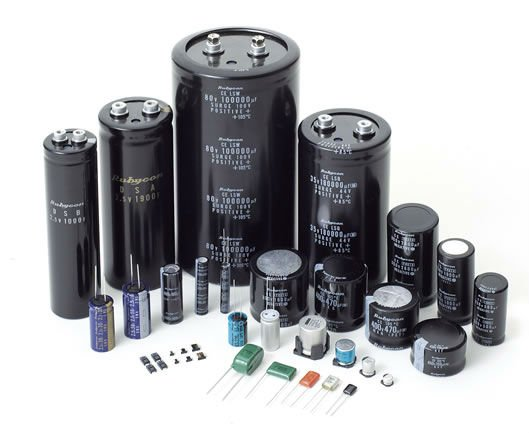
\includegraphics[width=0.5\linewidth]{Figuras/Ch16/capacitores.jpg}}
}

\frame{
	\frametitle{Definição}
	\begin{block}{Estrutura}
		Ele é constituído de duas peças condutoras que são chamadas de armaduras. Entre essas armaduras existe um material que é chamado de dielétrico (substância isolante que possui alta capacidade de resistência ao fluxo de corrente elétrica).
	\end{block}

	\centering
	\begin{tikzpicture}[scale=0.5]
			\draw (-4,-3) rectangle (4,3); %CLP
		\draw (-4,0) -- (-2.5,0); %Div in out
		\draw (-2.5,-3) -- (-2.5,3); %Div cartoes
		\draw (-1.5,-2.5) rectangle (0,2.5); %Mem dados
		\draw (0.5,-2.5) rectangle (3.5,-1); %Mem prog
		\draw (1,0) rectangle (3,2); %CPU
		\draw (-4,-5) rectangle (4,-3); %Alimentacao
		\draw (-2.5,4) rectangle (4,6); %Term de prog
		
		\draw (1,2.6) node {CLP};
		
		\draw (-3.25,1.5) node[text width=1.5cm,align=center,rotate=90] {\small Cartões de input};
		
		\draw (-3.25,-1.5) node[text width=1.5cm,align=center,rotate=90] {\small Cartões de output};
		
		\node at (2,1) {\small CPU};
		
		\node[rotate=90,text width=1.5cm,align=center] at (-0.75,0) {\small Memória de dados};
		
		\node[text width=2cm,align=center] at (2,-1.75) {\footnotesize Memória de programa};
		
		\node at (-6,0) {Campo};
		
		\node at (0,-4) {Alimentação};
		
		\node[text width=3cm,align=center] at (0.75,5) {Terminal de programação};
		
		\draw[-Latex] (-8,1.5) -- node[above] {Entradas} +(4,0);
		\draw[Latex-] (-8,-1.5) -- node[below] {Saídas} +(4,0);
		\draw[-Latex] (-2.5,1.5) -- +(1,0);
		\draw[Latex-] (-2.5,-1.5) -- +(1,0);
		\draw[-Latex] (0,1.5) -- +(1,0);
		\draw[Latex-] (0,0.5) -- +(1,0);
		\draw[Latex-] (2,0) -- +(0,-1);
		
		\draw[-Latex] (-1.5,4) -- +(0,-1);
		\draw[Latex-] (3,4) -- +(0,-1);
	\end{tikzpicture}
%	\centerline{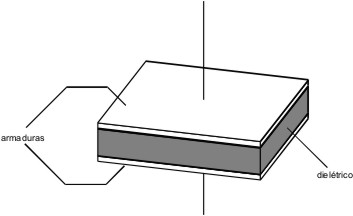
\includegraphics[width=0.5\linewidth]{Figuras/Ch16/armadura.jpg}}
}

\frame{
	\frametitle{Campo elétrico}
	\begin{block}{Funcionamento}
		Este equipamento é construído utilizando um campo elétrico uniforme. Para que haja um campo elétrico uniforme é necessário que haja uma interação específica, limitando os possíveis formatos geométricos de um capacitor.
	\end{block}

	\begin{minipage}{0.49\linewidth}
		\centering
		
		\setmyunit{1cm}
		\begin{tikzpicture}
		\filldraw[fill=black!80!white] (0,0) rectangle (2,0.15);
		\filldraw[fill=black!40!white] (0.1,0.15) -- ++(0,1) -- ++(0.2,0)
		-- ++(0,0.2) -- ++(0.15,0) node[below] {\small $ + $} node[coordinate,name=p1] {} -- ++(0.15,0) -- ++(0,-0.2)
		-- ++(0.8,0)
		-- ++(0,0.2) -- ++(0.15,0) node[below] {\small $ - $} node[coordinate,name=p2] {} -- ++(0.15,0) -- ++(0,-0.2)
		-- ++(0.2,0) -- ++(0,-1) -- cycle;
		
		\draw[thin] (p1) -- ++(0,0.3) -- ++(-0.5,0) -- ++(0,0.3) -- ++(0.3,0) ++(0,-0.2) rectangle +(0.4,2) (p2) -- ++(0,0.3) -- ++(0.5,0) -- ++(0,0.3) -- ++(-0.3,0) ++(-0.4,-0.2) rectangle +(0.4,2);
		
		\foreach \x in {0.25,0.5,...,1.75} {
			\draw ($ (p1)+(0,0.4) $) +(0,\x) node {$ + $};
			\draw ($ (p2)+(0,0.4) $) +(0,\x) node {$ - $};
			\draw[->] ($ (p1)+(0.2,0.4)+(0,\x) $) -- ($ (p2)+(-0.2,0.4)+(0,\x) $);
		}
		
		\draw ($ (p1)!0.5!(p2) $) +(0,2.4) node {$ \vec{E} $};
		
		\node[] at (1,0.675) {Bateria};
		\end{tikzpicture}
		
%		\centerline{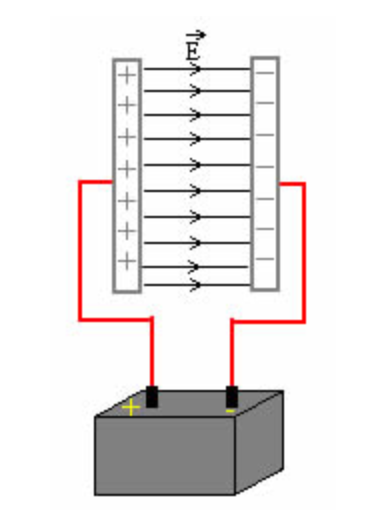
\includegraphics[width=0.65\linewidth]{Figuras/Ch16/campo.PNG}}
	\end{minipage}
	\hfill
	\begin{minipage}{0.5\linewidth}
		%\scriptsize
		\begin{equation*}
			\boxed{E = \dfrac{U}{d}}
		\end{equation*}
		onde: \\
		$E$ = campo elétrico \\
		$U$ = diferença de potencial aplicado \\
		$d$ = distância entre as placas \\
	\end{minipage}
}

\frame{
	\frametitle{Capacitância}
	\begin{block}{Relação matemática}
		É denominada capacitância $ C $ a \textbf{propriedade} que os capacitores têm de armazenar cargas elétricas na forma de campo eletrostático, e ela é medida através do quociente entre a quantidade de carga ($Q$) e a diferença de potencial ($U$) existente entre as placas do capacitor.
	\end{block}
	$$\boxed{C = \dfrac{Q}{U}}$$
	\begin{block}{Unidade de medida}
		No SI, a unidade de capacitância é o \textbf{farad} (\si{\farad})
		\begin{itemize}
			\item microfarads (\si{\micro\farad})
			\item nanofarads \ (\si{\nano\farad})
			\item picofarads \ \ (\si{\pico\farad})
		\end{itemize}
	\end{block}
}

\frame{
	\frametitle{Capacitores planos}
	\begin{block}{Capacitância}
		O capacitor plano é um dispositivo feito por duas placas de metal. Essas placas precisam necessariamente ser iguais e planas, ter o mesmo tamanho e estar próximas uma da outra. Entre elas é colocado o dielétrico, um isolante.
	\end{block}
	\begin{minipage}{0.4\textwidth}
		\centering
		\begin{tikzpicture}[scale=0.5]
			\draw (-4,-3) rectangle (4,3); %CLP
		\draw (-4,0) -- (-2.5,0); %Div in out
		\draw (-2.5,-3) -- (-2.5,3); %Div cartoes
		\draw (-1.5,-2.5) rectangle (0,2.5); %Mem dados
		\draw (0.5,-2.5) rectangle (3.5,-1); %Mem prog
		\draw (1,0) rectangle (3,2); %CPU
		\draw (-4,-5) rectangle (4,-3); %Alimentacao
		\draw (-2.5,4) rectangle (4,6); %Term de prog
		
		\draw (1,2.6) node {CLP};
		
		\draw (-3.25,1.5) node[text width=1.5cm,align=center,rotate=90] {\small Cartões de input};
		
		\draw (-3.25,-1.5) node[text width=1.5cm,align=center,rotate=90] {\small Cartões de output};
		
		\node at (2,1) {\small CPU};
		
		\node[rotate=90,text width=1.5cm,align=center] at (-0.75,0) {\small Memória de dados};
		
		\node[text width=2cm,align=center] at (2,-1.75) {\footnotesize Memória de programa};
		
		\node at (-6,0) {Campo};
		
		\node at (0,-4) {Alimentação};
		
		\node[text width=3cm,align=center] at (0.75,5) {Terminal de programação};
		
		\draw[-Latex] (-8,1.5) -- node[above] {Entradas} +(4,0);
		\draw[Latex-] (-8,-1.5) -- node[below] {Saídas} +(4,0);
		\draw[-Latex] (-2.5,1.5) -- +(1,0);
		\draw[Latex-] (-2.5,-1.5) -- +(1,0);
		\draw[-Latex] (0,1.5) -- +(1,0);
		\draw[Latex-] (0,0.5) -- +(1,0);
		\draw[Latex-] (2,0) -- +(0,-1);
		
		\draw[-Latex] (-1.5,4) -- +(0,-1);
		\draw[Latex-] (3,4) -- +(0,-1);
	\end{tikzpicture}
%		\centerline{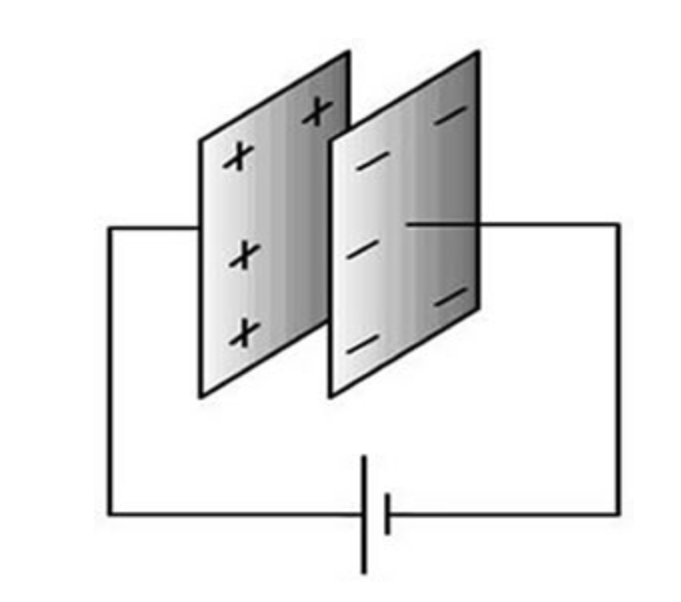
\includegraphics[width=0.9\linewidth]{Figuras/Ch16/plano.PNG}}
	\end{minipage}%%% to prevent a space
	\begin{minipage}{0.6\textwidth}
		\vspace{0.5cm}
		%\scriptsize
		\begin{equation*}
			\boxed{C = \varepsilon \dfrac{A}{d}}
		\end{equation*}
		onde: \\
		$C$ = capacitância [\si{\farad}] \\
		$\varepsilon$ = permissividade do meio isolante [\si{\farad\per\meter}] \\
		$A$ = área [\si{\meter\squared}] \\
		$d$ = distância entre as placas [\si{\meter}]
	\end{minipage}
}

\frame{
	\frametitle{Circuito elétrico}
	\begin{block}{Simbologia}
		$$\begin{circuitikz}[scale=1.25]
				\ctikzset{label/align=smart,bipoles/length=1.5cm}
				\draw (0,0) to[C,l_=\mbox{$C$},*-*] (2,0);
			\end{circuitikz}$$
	\end{block}
}

\frame{
	\frametitle{Aplicação}
	\begin{block}{Exemplo}
		\begin{itemize}
			\item Flash de uma câmera
		\end{itemize}
	\end{block}
	\centerline{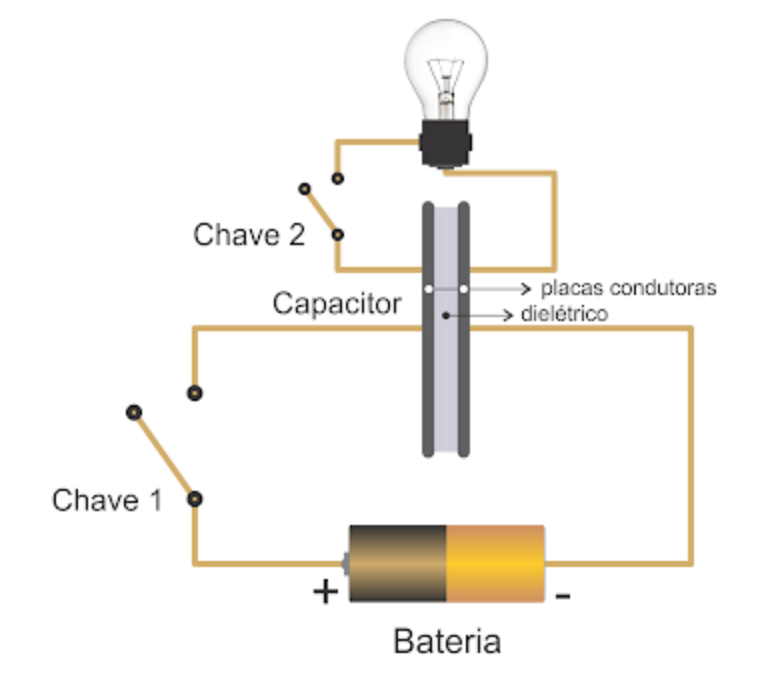
\includegraphics[width=0.5\linewidth]{Figuras/Ch16/flash.png}}
}

\frame{
	\frametitle{Capacitores}
	\begin{block}{Exemplo \#01}
		(UFV-2005) Duplicando-se a diferença de potencial entre as placas de um capacitor, é CORRETO afirmar que: \vspace{0.5cm}

		(a) a carga e a capacitância do capacitor também são duplicadas. \vspace{0.2cm}

		(b) a carga e a capacitância do capacitor permanecem constantes. \vspace{0.2cm}

		(c) a carga do capacitor é duplicada, mas sua capacitância permanece constante. \vspace{0.2cm}

		(d) a carga e a capacitância do capacitor são reduzidas à metade dos valores iniciais. \vspace{0.2cm}

		(e) a carga do capacitor é duplicada, e sua capacitância é dividida pela metade. \vspace{0.2cm}
	\end{block}
}

\frame{
	\frametitle{Capacitores}
	\begin{block}{Exemplo \#02}
		Entre as placas dos capacitores, costuma-se inserir um material dielétrico preferencialmente ao vácuo. A inserção de um material dessa natureza entre as placas de um capacitor: \vspace{0.5cm}

		(a) aumenta a sua capacitância por causa da sua maior permissividade elétrica. \vspace{0.2cm}

		(b) aumenta a sua capacitância, diminuindo a quantidade de cargas entre as suas placas. \vspace{0.2cm}

		(c) não afeta a sua capacitância. \vspace{0.2cm}

		(d) diminui a sua capacitância, por causa da sua maior permissividade elétrica. \vspace{0.2cm}

		(e) não afeta a formação do campo elétrico entre as placas do capacitor. \vspace{0.2cm}
	\end{block}
}

\frame{
	\frametitle{Capacitores}
	\begin{block}{Exemplo \#03}
		Em relação à capacitância de um capacitor de placas paralelas, assinale o que for FALSO: \vspace{0.5cm}

		(a) a capacitância é diretamente proporcional à área dos capacitores. \vspace{0.2cm}

		(b) a capacitância é inversamente proporcional à distância entre os capacitores. \vspace{0.2cm}

		(c) a permissividade elétrica é uma característica que depende do material inserido entre as placas do capacitor. \vspace{0.2cm}

		(d) quanto maior for a capacitância de um capacitor, menos carga ele pode armazenar para uma determinada tensão elétrica. \vspace{0.2cm}

		(e) quanto menor for a capacitância de um capacitor, menos carga ele pode armazenar para uma determinada tensão elétrica. \vspace{0.2cm}
	\end{block}
}

\frame{
	\frametitle{Energia armazenada em um capacitor}
	\begin{block}{Conceito}
		A grande utilidade dos capacitores reside no fato de que esses dispositivos podem armazenar energia ao manter uma diferença de potencial entre suas placas, em virtude da separação de cargas.
	\end{block}
	\centerline{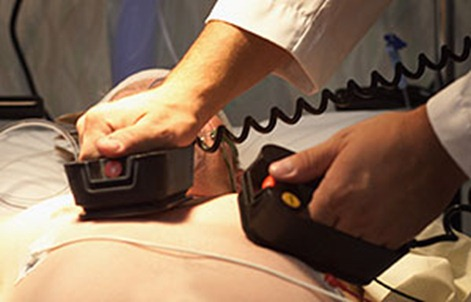
\includegraphics[width=0.5\linewidth]{Figuras/Ch16/desf.jpg}}
}

\frame{
	\frametitle{Energia armazenada em um capacitor}
	\begin{block}{Conceito}
		\begin{itemize}
			\item À medida que o capacitor é carregado por cargas, ele acumula energia potencial elétrica.
			\item A energia necessária para carregar o capacitor corresponde, numericamente, à área sob a curva.
		\end{itemize}
	\end{block}

	\vspace{0.2cm}

	\begin{minipage}{0.5\textwidth}
%		\vspace{0.5cm}
		\centering
		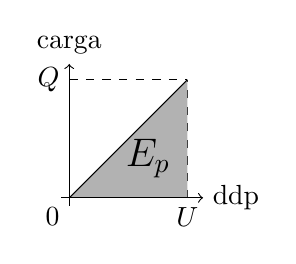
\begin{tikzpicture}
			\draw (0,0) node[below left] {$ 0 $};
			\draw[dashed] (0,1.5) node[left] {$ Q $} -- (1.5,1.5);
			\draw[dashed] (1.5,0) node[below] {$ U $} -- (1.5,1.5);
			\fill[black!30] (0,0) -- (1.5,0) -- (1.5,1.5) -- cycle;
			\draw (1,0.5) node[] {\Large $ E_p $};
			
			\draw[->] (-0.1,0) -- (1.7,0) node[right] {ddp};
			\draw[->] (0,-0.1) -- (0,1.7) node[above] {carga};
			\draw (0,0) -- (1.5,1.5);
		\end{tikzpicture}
%		\centerline{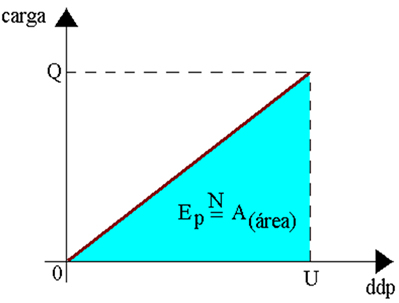
\includegraphics[width=0.9\linewidth]{Figuras/Ch16/ept.jpg}}
	\end{minipage}%%% to prevent a space
	\begin{minipage}{0.5\textwidth}
%		\vspace{0.5cm}
		%\scriptsize
		\begin{equation*}
			\boxed{E_p = \dfrac{Q \cdot U}{2} = \dfrac{C \cdot U^2}{2}}
		\end{equation*}
	\end{minipage}
}

\frame{
	\frametitle{Associação de capacitores}
	\begin{block}{Série}
		\begin{itemize}
			\item Na associação em série a armadura negativa do capacitor está ligada a armadura positiva do capacitor seguinte.
			\item Quando os capacitores são ligados em série a \textbf{carga da associação é igual para todos os capacitores}.
		\end{itemize}
	\end{block}

	\medskip

	\centering
	\setmyunit{2cm}
	\begin{circuitikz}
		\foreach \x in {1,2,3,4}{
			\draw ($ (\x,0)+(-1,0) $) to[C,l=$ C_{\x} $,*-*] ++(1,0);
%			\draw[<->] ($ (\x,-0.5)+(-1,0) $) -- node[below] {$ Q_{\x} $} ++(1,0);
%			\draw[dashed] ($ (\x,0)+(-1,0) $) -- ++(0,-0.6);
		}
		
		\draw[<->] (-0.04,-0.5) -- node[below] {$ C_{eq} $} ++(4.08,0);
		\draw[dashed] (-0.04,0) -- ++(0,-0.6);
		\draw[dashed] (4.04,0) -- ++(0,-0.6);
	\end{circuitikz}

%	\centerline{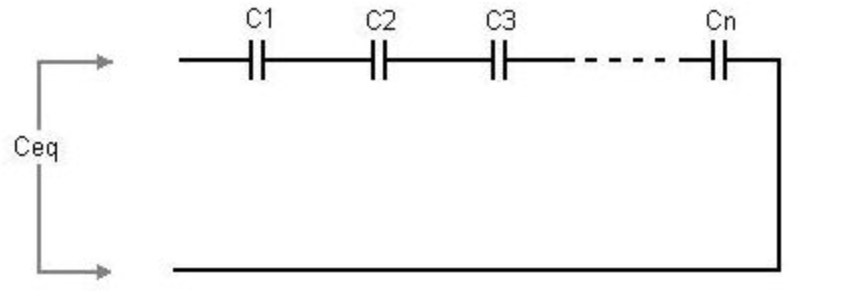
\includegraphics[width=0.8\linewidth]{Figuras/Ch16/capacitorserie.PNG}}
}

\frame{
	\frametitle{Associação de capacitores}
	\begin{block}{Série}
		Com três capacitores:

		$$V_1 = \dfrac{Q}{C_1} \qquad V_2 = \dfrac{Q}{C_2} \qquad V_3 = \dfrac{Q}{C_3}$$

		Como $V = V_1 + V_2 + V_3$,
		\begin{align*}
			\dfrac{Q}{C_{eq}} &= \dfrac{Q}{C_1} + \dfrac{Q}{C_2} + \dfrac{Q}{C_3} \Rightarrow\\
			\dfrac{1}{C_{eq}} &= \dfrac{1}{C_1} + \dfrac{1}{C_2} + \dfrac{1}{C_3}
		\end{align*}
		
		Generalizando...

		$$\boxed{\dfrac{1}{C_{eq}} = \dfrac{1}{C_1} + \dfrac{1}{C_2} + \dfrac{1}{C_3} + ... + \dfrac{1}{C_n}}$$
	\end{block}
}

\frame{
	\frametitle{Associação de capacitores}
	\begin{block}{Paralelo}
		\begin{itemize}
			\item Na associação de capacitores em paralelo as armadura negativas do capacitor são ligadas entre si assim como as  armaduras positivas  do capacitor.
			\item Quando os capacitores são ligados em paralelo a \textbf{ddp da associação é a mesma para todos os capacitores}.
		\end{itemize}
	\end{block}

	\bigskip

	\centering
	\setmyunit{2cm}
	\begin{circuitikz}
		\draw (0,0) to[short,o-*] ++(1,0)
		to[C,l=$ C_1 $] ++(0,-1)
		to[short,*-o] ++(-1,0)
		(1,0) -- ++(1,0)
		to[C,l=$ C_2 $,*-*] ++(0,-1) -- ++(-1,0)
		(3,0)	to[C,l=$ C_n $] ++(0,-1);
		
		\draw (2,0) -- (2.5,0) (2.7,0) -- (3,0) (2,-1) -- (2.5,-1) (2.7,-1) -- (3,-1);
		\draw[dotted] (2.5,0) -- (2.7,0) (2.5,-1) -- (2.7,-1);
		\draw (2.6,-0.5) node {$ \cdots $};
	\end{circuitikz}
%	\centerline{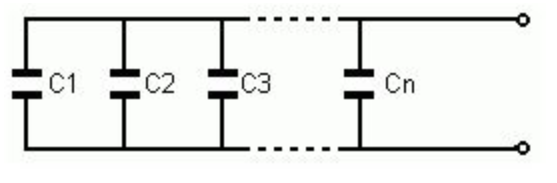
\includegraphics[width=0.8\linewidth]{Figuras/Ch16/capacitorparalelo.PNG}}
}

\frame{
	\frametitle{Associação de capacitores}
	\begin{block}{Paralelo}
		$$Q_1 = C_1U \qquad Q_2 = C_2U \qquad Q_3 = C_3U$$
		
		Como $Q = Q_1 + Q_2 + Q_3$,
		\begin{align*}
			C_{eq}U &= C_1U + C_2U + C_3U \Rightarrow \\
			C_{eq} &= C_1 + C_2 + C_3
		\end{align*}
	
		Generalizando...
		
		$$\boxed{C_{eq} = C_1 + C_2 + C_3 + ... + C_n}$$
	\end{block}
}

\frame{
	\frametitle{Associação de capacitores}
	\begin{block}{Mista - Exemplo \#01}
		\begin{itemize}
			\item Neste tipo de associação encontramos capacitores associadas em \textbf{série} e em \textbf{paralelo}.
%			      \vspace{1cm}
			\item Para $C_1 = \SI{2}{\micro\farad}$, $C_2 = \SI{3}{\micro\farad}$ e $C_3 = \SI{5}{\micro\farad}$, calcule a capacitância equivalente da associação da figura abaixo.
		\end{itemize}
	\end{block}

	\centering
	\setmyunit{2cm}
	
	\begin{circuitikz}
		\draw (0,0) to[short,o-*] ++(0.5,0) -- ++(0,0.5)
		to[C,l=$ C_1 $] ++(1,0) -- ++(0,-1)
		to[C,l_=$ C_2 $] ++(-1,0) -- ++(0,0.5)
		(1.5,0) to[C,l=$ C_3 $,*-o] ++(1,0);
	\end{circuitikz}
%	\centerline{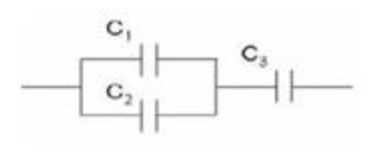
\includegraphics[width=0.5\linewidth]{Figuras/Ch16/capacitormista.PNG}}
}

\section*{Exercícios}

\frame{
	\frametitle{Exercícios}
	\begin{block}{}

		01. Um capacitor plano é constituído por duas placas metálicas planas e paralelas distantes \SI{20}{\centi\meter} uma da outra, apresentando uma área $A = \SI{0.10}{\meter\squared}$. O meio entre elas é o ar, que tem permissividade absoluta aproximadamente igual à do vácuo ($\varepsilon = \SI{8.8e-12}{\farad\per\meter})$. Este capacitor é ligado a uma bateria com tensão $V = \SI{50}{\volt}$. Determine:

		(a) a capacitância desse capacitor. \\
		(b) a carga elétrica armazenada. \\
		(c) a intensidade do campo elétrico.

		\vspace{0,5cm}


		02. Três capacitores são ligados em série. A capacitância do primeiro é expressa por $C_1 = \SI{5}{\micro\farad}$, assim segue $C_2 = \SI{3}{\micro\farad}$ e $C_3 = \SI{7}{\micro\farad}$. Esta associação está combinada por uma ddp de \SI{12}{\volt}. Pede-se:

		(a) a capacitância equivalente. \\
		(b) A carga de cada capacitor. \\
		(c)  A diferença de potencial elétrico de cada capacitor.
	\end{block}
}


\section*{Referências}

\frame{
	\frametitle{Referências e Exercícios Complementares}
	\begin{itemize}
		\item Física, Ciência e Tecnologia – Vol 3. PENTEADO, Paulo César M; TORRES, Carlos Magno A. Ed. Moderna (2006)
	\end{itemize}
	%\centering{\alert{Página 36 - \textbf{1.6.1 até 1.6.5, 1.6.17 até 1.6.19}}} \\
	\centering{\alert{Lista de exercícios 16}}
}